\documentclass{beamer}
\usetheme{Boadilla}
\usepackage[utf8x]{inputenc}
\usepackage{listings}
\usepackage{subfig}
%\title{LS Genio Platform}
%\subtitle{Piattaforma per il monitoraggio di macchine utensili con integrazione a software ERP Microsoft Dynamics NAV}
%\author{Vincenzo Nucci e Matteo Tiberi}
%\author{Matteo Tiberi}
%\institute{Università di Camerino}
\date{}
\begin{document}
	
	\begin{frame}
	\centering
	
\includegraphics[scale=0.25]{images/frontespizio-beamer.png}\par
	\usebeamertemplate{title page}
\end{frame}

\begin{frame}
	\frametitle{Obiettivi}
		\begin{itemize}
			\item Piattaforma REST indipendente da sorgenti dati
			\begin{itemize}
				\item Autenticazione tramite token
				\item Interfaccia web
			\end{itemize}
			\item Servizio di sottoscrizione "subscribe"
			\begin{itemize}
				\item Notifica dei messaggi PUSH
			\end{itemize}
			\item Integrazione dei servizi con NAV
			\item Servizio di monitoraggio dei dati
			\begin{itemize}
				\item Controllo valore oltre soglia
			\end{itemize}
		\end{itemize}
\end{frame}

\begin{frame}
\frametitle{Architettura piattaforma}
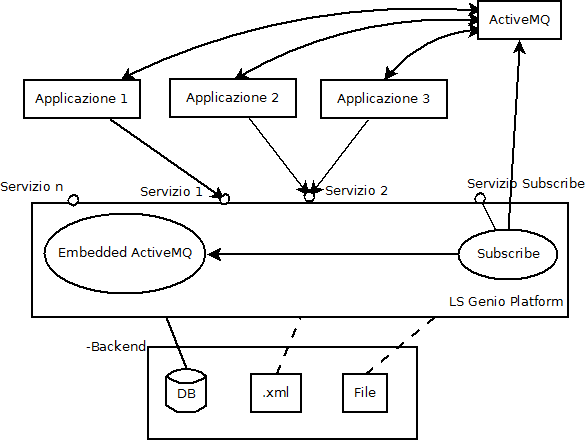
\includegraphics[width=0.9\textwidth]{images/architettura_piattaforma.png}
\end{frame}

\begin{frame}
\frametitle{Struttura tabelle backend}
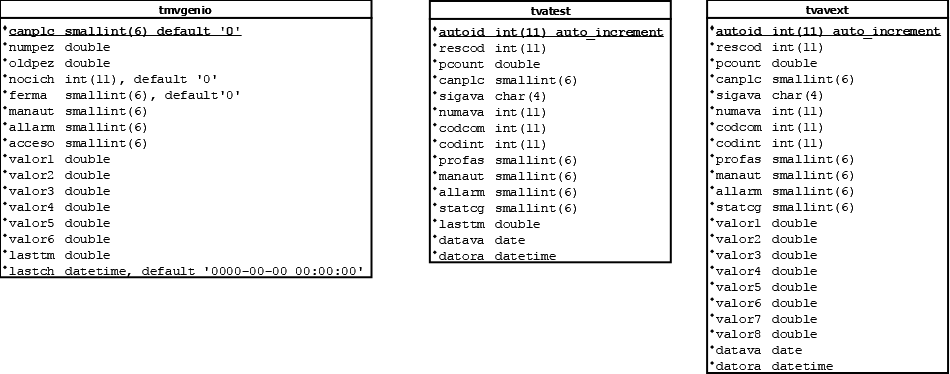
\includegraphics[width=1\textwidth]{images/tabelle-backend.png}
\end{frame}

\begin{frame}
\frametitle{Pagina web per la richiesta di abilitazione}
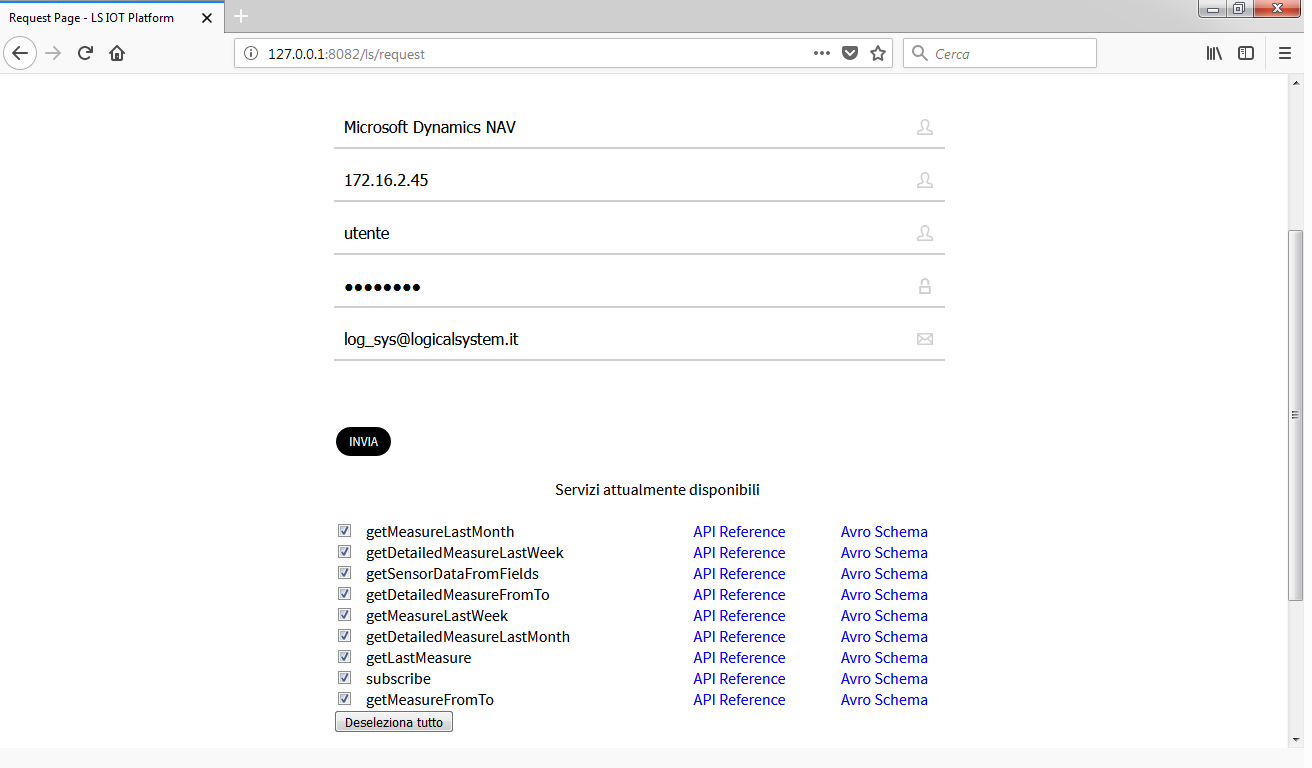
\includegraphics[width=1\textwidth]{images/RequestPagePlatform.png}
\end{frame}

\begin{frame}
\frametitle{Pagina web catalogo Smart Object}
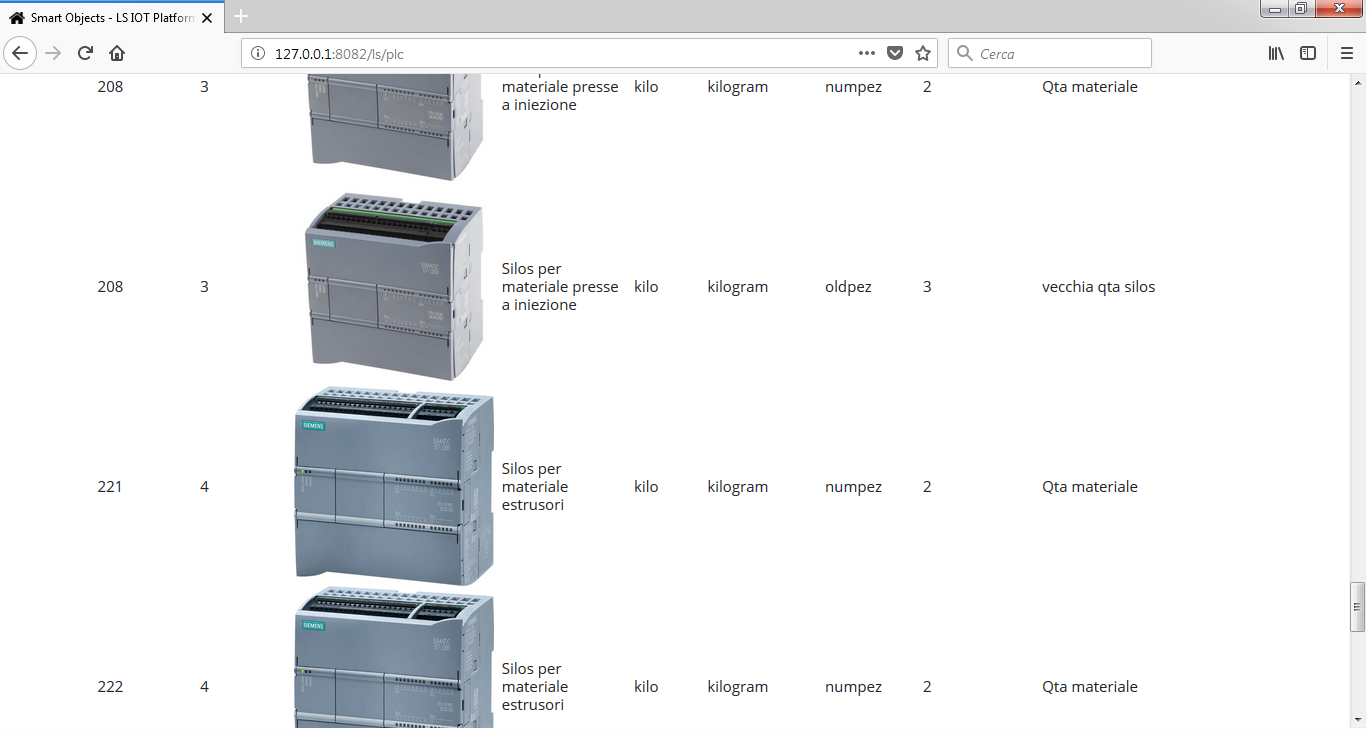
\includegraphics[width=1\textwidth]{images/SmartObjectsPlatform.png}
\end{frame}

\begin{frame}
\frametitle{Esempio di un servizio - getlastmeasure}
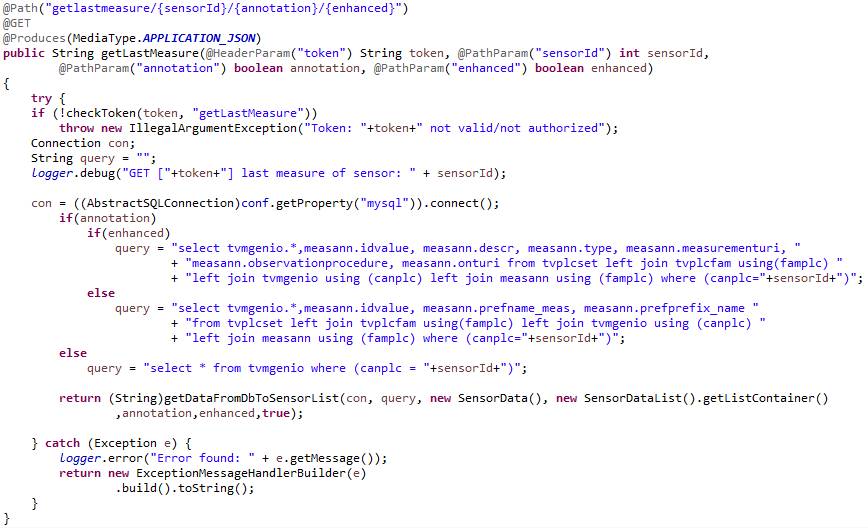
\includegraphics[width=1\textwidth]{images/getlastmeasure.png}
\end{frame}

\begin{frame}
\frametitle{Valori di ritorno di getlastmeasure}
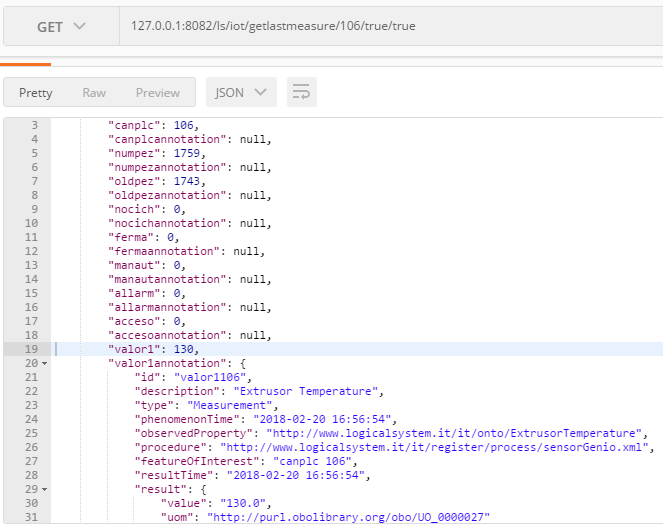
\includegraphics[width=0.8\textwidth]{images/Postman1-corretto.png}
\end{frame}

\begin{frame}
\frametitle{Subscribe Rule di una applicazione}
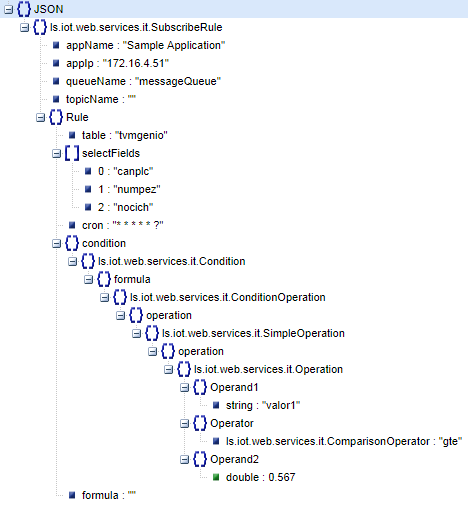
\includegraphics[width=0.6\textwidth]{images/subscribe-json-1.png}
\end{frame}

\begin{frame}
\frametitle{Albero della condition}
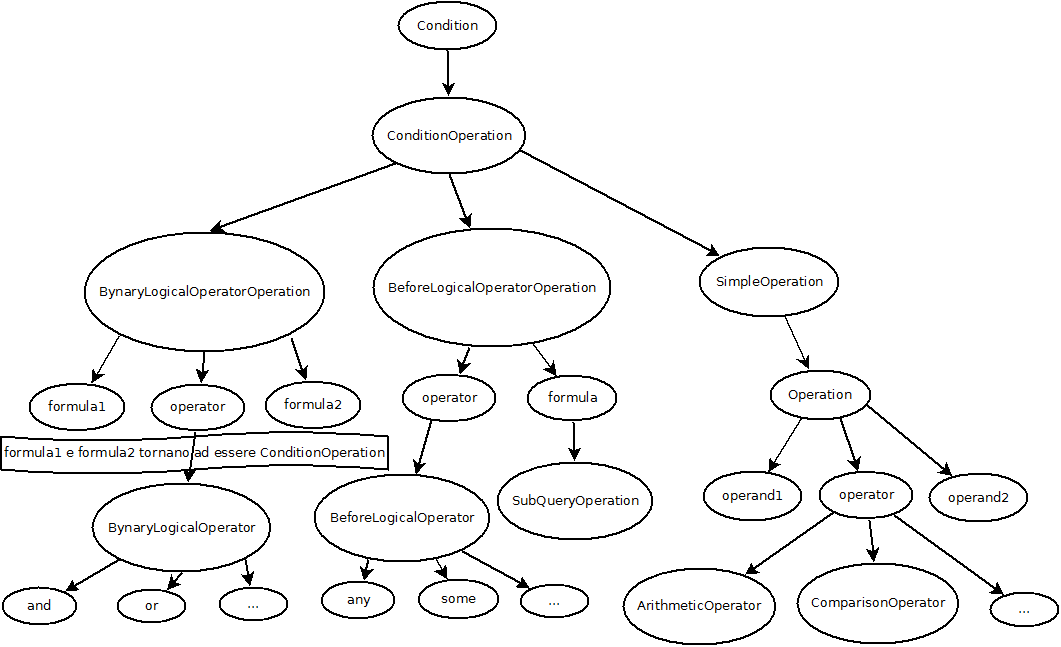
\includegraphics[width=1\textwidth]{images/strutturaquerytree.png}
\end{frame}

\begin{frame}
\frametitle{Class Diagram SubscribeRuleInterface}
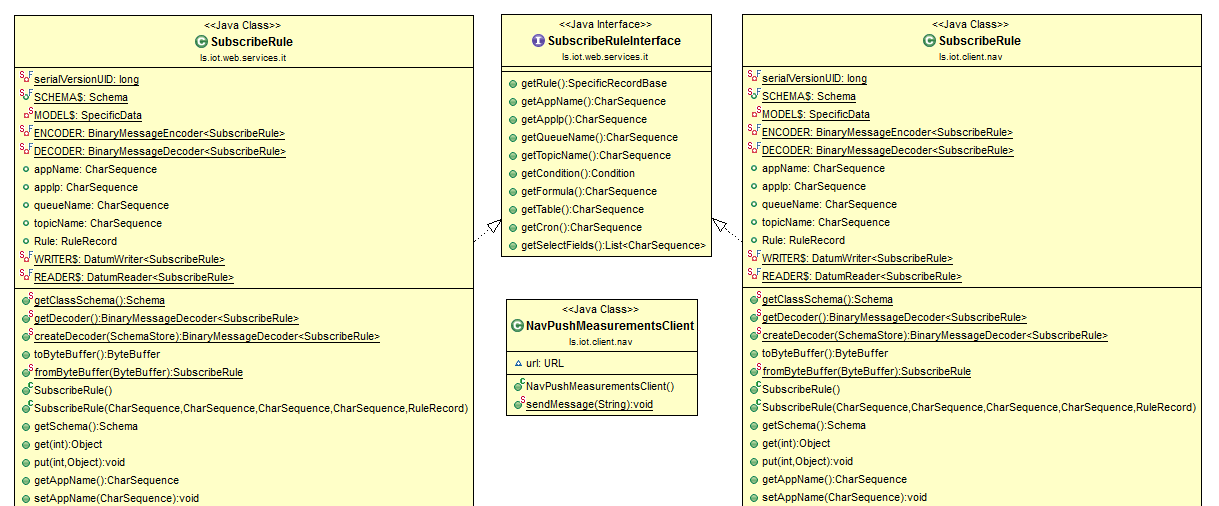
\includegraphics[width=1\textwidth]{images/figura10.png}
\end{frame}

\begin{frame}
\frametitle{Class Diagram RetrievedDataInterface}
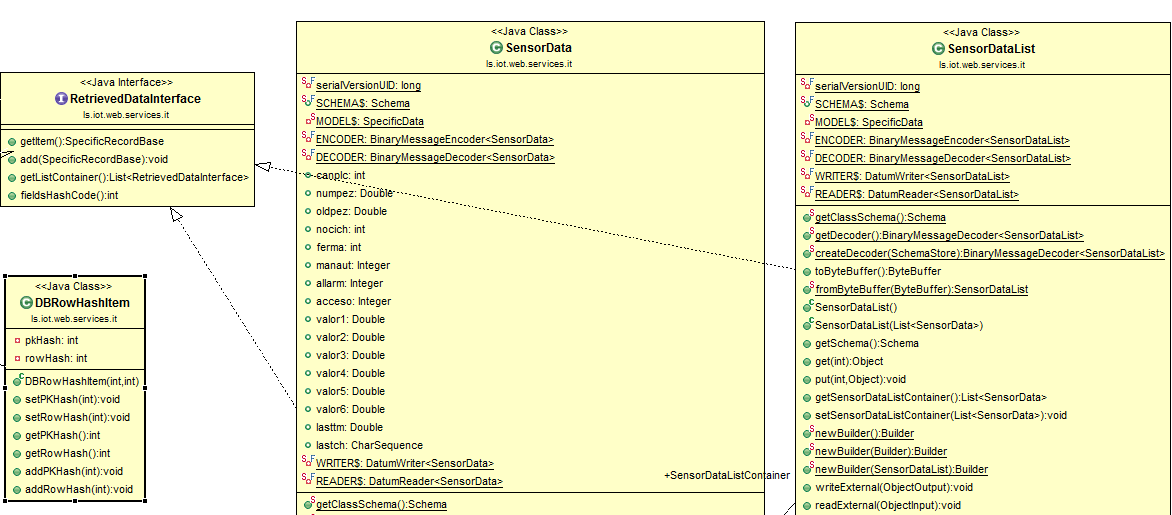
\includegraphics[width=1\textwidth]{images/ClassDiagram1.png}
\end{frame}

\begin{frame}
\frametitle{Class Diagram AnnotationInterface}
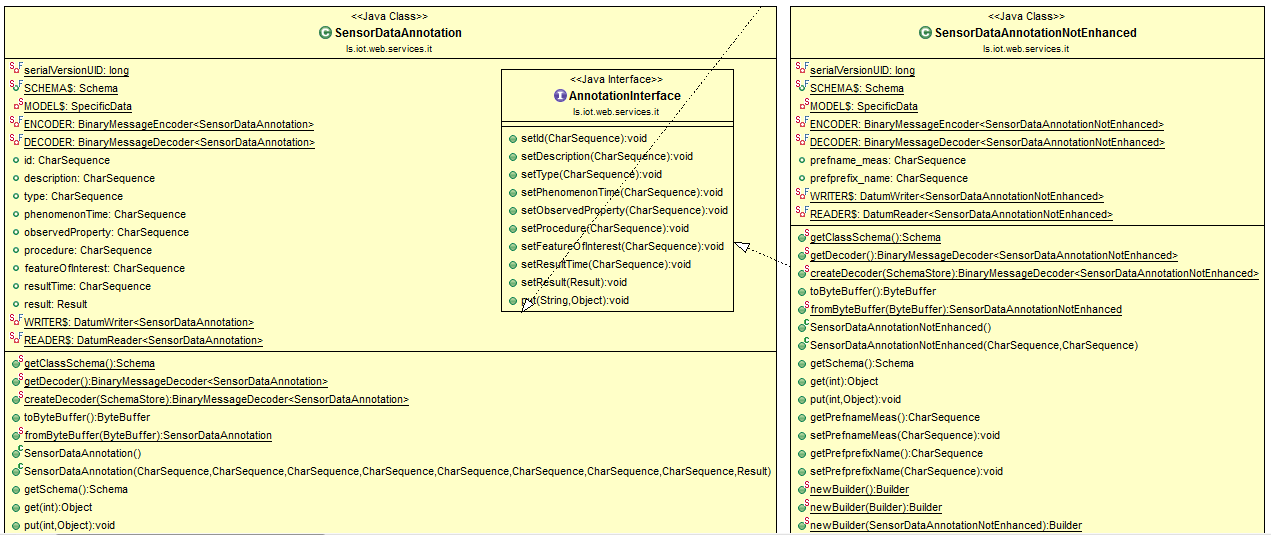
\includegraphics[width=1\textwidth]{images/annotationinterface.png}
\end{frame}

\begin{frame}
\frametitle{Class Diagram AbstractConnection}
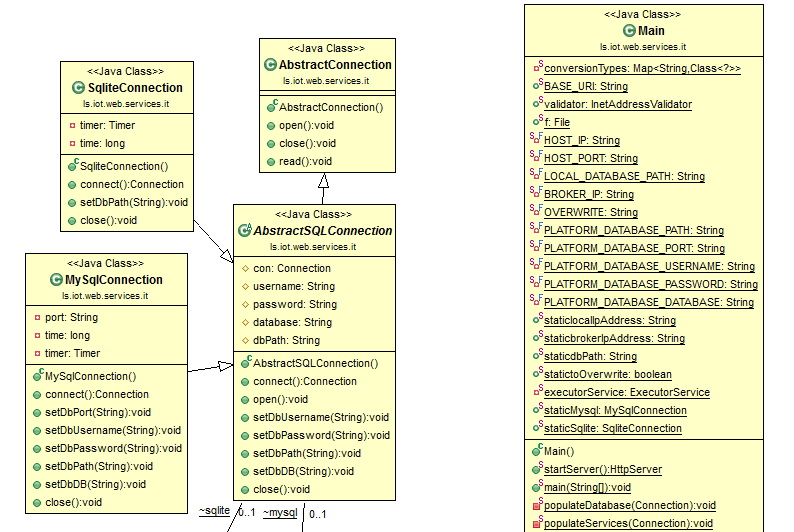
\includegraphics[width=1\textwidth]{images/main.png}
\end{frame}

\begin{frame}
\frametitle{Schema Avro SensorData}
\begin{figure}%
	\centering
	\subfloat{{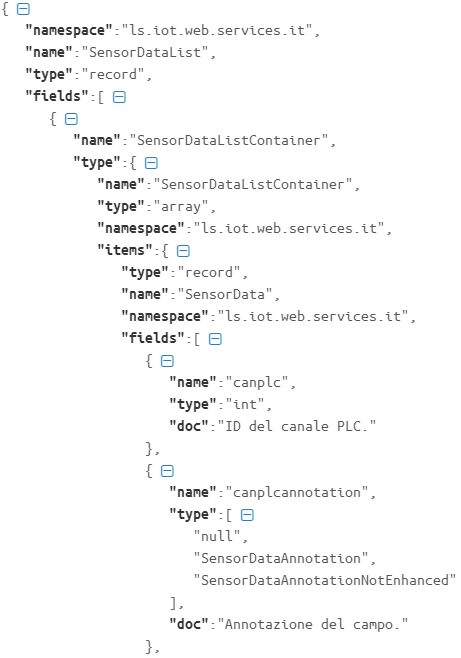
\includegraphics[width=5cm]{images/sensordata1.png} }}%
	\qquad
	\subfloat{{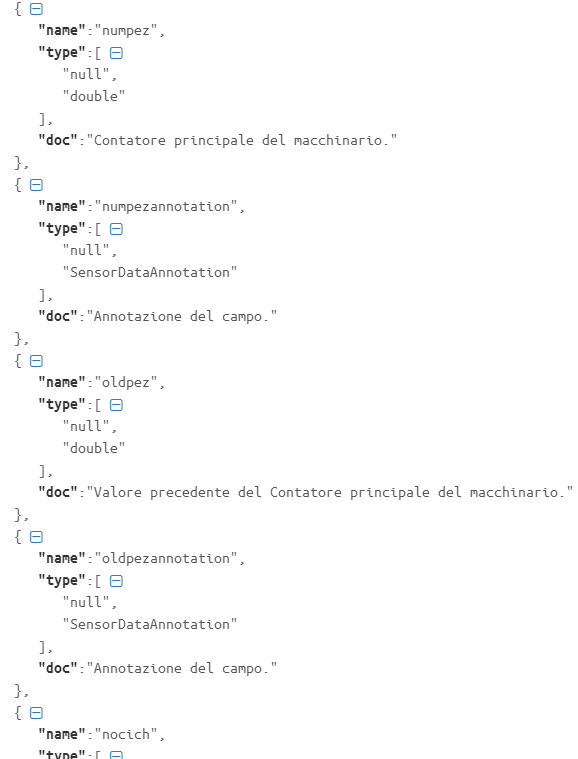
\includegraphics[width=6cm]{images/sensordata2.png} }}%
	%
	%
\end{figure}
\end{frame}

\begin{frame}
\frametitle{Schema Avro SensorDataAnnotation}
\begin{figure}%
	\centering
	\subfloat{{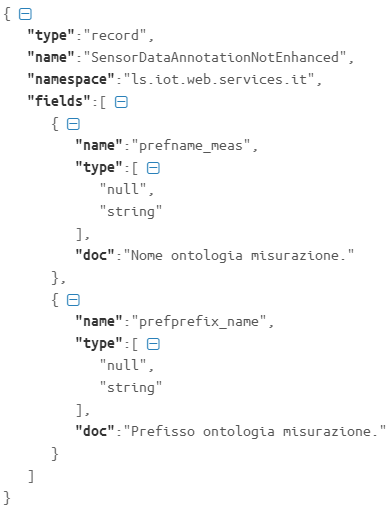
\includegraphics[width=5cm]{images/annotazione-non-avro.png} }}%
	\qquad
	\subfloat{{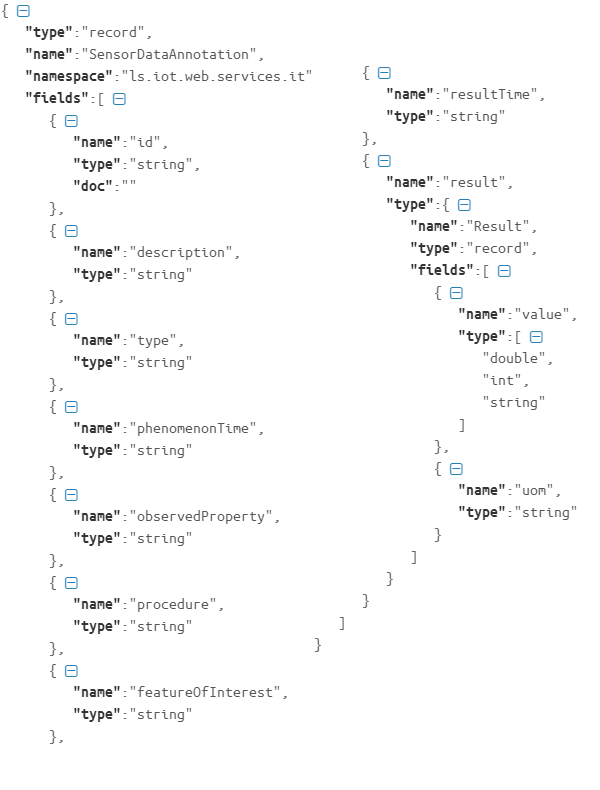
\includegraphics[width=6cm]{images/annotazione-avro.png} }}%
	%
	%
\end{figure}
\end{frame}

\begin{frame}
\frametitle{Pagina web per il grafico}
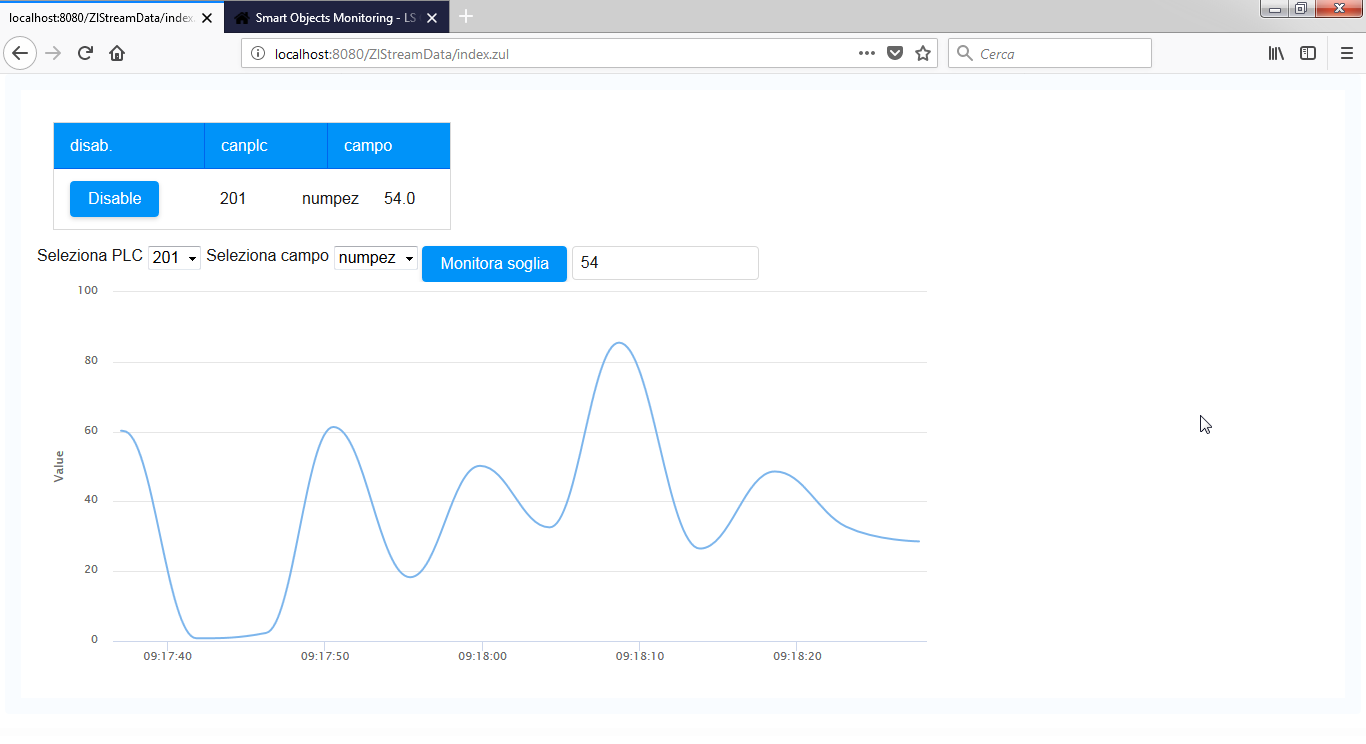
\includegraphics[width=1\textwidth]{images/grafico-zk.png}
\end{frame}

\begin{frame}
\frametitle{Codice Job Flink}
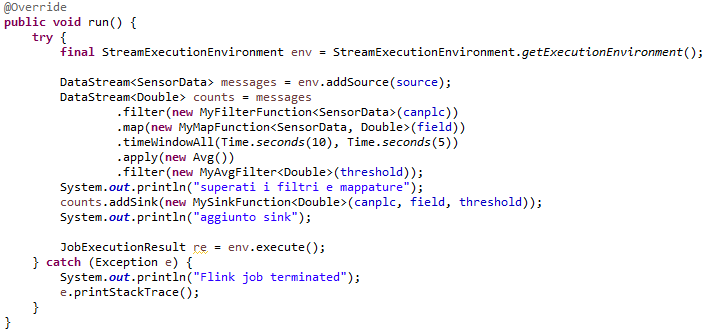
\includegraphics[width=1\textwidth]{images/flink-job.png}
\end{frame}

\begin{frame}
\frametitle{Difficoltà incontrate}
\begin{itemize}
	\item Integrazione subscribe con NAV
	\begin{itemize}
		\item Utilizzo Web Service SOAP
	\end{itemize}
\end{itemize}
\end{frame}

\begin{frame}
\frametitle{Tecnologie utilizzate}
\begin{itemize}
	\item Java
	\item Framework Jersey e Grizzly
	\item Apache Avro
	\item Apache ActiveMQ
	\item Framework ZK
	\item Apache Flink
\end{itemize}
\end{frame}

\begin{frame}
\frametitle{Risultati raggiunti}
\begin{itemize}
	\item Piattaforma indipendente
	\begin{itemize}
		\item Classi astratte e interfacce
		\item Database SQLite per autenticazione token
	\end{itemize}
	\item Servizio subscribe debolmente accoppiato
	\begin{itemize}
		\item Tramite message broker
	\end{itemize}
	\item Servizio monitoraggio dei dati
	\begin{itemize}
		\item Grafico per visualizzare andamento
		\item Apache Flink per controllo soglia
	\end{itemize}
\end{itemize}
\end{frame}

%-------------------------inizio client-----------------------------

\begin{frame}
\frametitle{Obiettivi}
\begin{itemize}
	\item Interazione di Microsoft Dynamics NAV con la piattaforma LS-Genio Mashup e definizione di un "setup" per l'utente
	%\begin{itemize}
	%	\item Mancata possibilità di consumo diretto di servizi REST
	%	\item Mancata possibilità di gestione del formato JSON
	%	\item Difficoltà nell'interazione con software esterni non Microsoft
	%\end{itemize}
	
	%\item Visualizzazione tramite NAV di un report PowerBI basato sui dati ottenuti
	
	%\item Visualizzazione da NAV di una rappresentazione grafica con PowerBI dei dati ottenuti 
	\item Realizzazione di un ontologia delle misurazioni e delle misure
\end{itemize}	
\end{frame}

\begin{frame}
\frametitle{Problematiche e risoluzioni}
\begin{itemize}
\item Software Microsoft Dynamics NAV che possiede numerose limitazioni, ostacolando l'interazione con la piattaforma
\begin{itemize}
	\item Risolto mediante implementazione di un client C\#, integrato poi su NAV
	%	\item Mancata possibilità di gestione del formato JSON
	%	\item Difficoltà nell'interazione con software esterni non Microsoft
\end{itemize}

%	\item Impossibilità di integrare un report PowerBI su NAV senza l'utilizzo di Azure
%	\begin{itemize}
%		\item Risolto mediante esportazione del report su Web
%	\end{itemize}

\item Difficoltà nel trovare un modello ontologico relativo al case study
\begin{itemize}
	\item Risolto mediante adattamento allo standard ISO 19156:2011
\end{itemize}
\end{itemize}	
\end{frame}

\begin{frame}
\frametitle{Tecnologie e software utilizzati}
\begin{itemize}
\item C\#
\item Apache Avro
\item Microsoft Dynamics NAV e C/AL code%(C/SIDE e RoleTailored Client)
\item Microsoft PowerBI
\item Protégé
\item MySQL
%\begin{itemize}
%	\item Mancata possibilità di consumo diretto di servizi REST
%	\item Mancata possibilità di gestione del formato JSON
%	\item Difficoltà nell'interazione con software esterni non Microsoft
%\end{itemize}
\end{itemize}	
\end{frame}

%\begin{frame}
%\frametitle{Client per la piattaforma}
%\begin{itemize}
%\item Sviluppato su Microsoft Dynamics NAV nonostante diverse lacune dell'ambiente
%\begin{itemize}
%\item Mancata possibilità di consumo diretto di servizi REST
%\item Mancata possibilità di gestione del formato JSON
%\item Difficoltà nell'interazione con software esterni non Microsoft
%\end{itemize}
%\item Risoluzione tramite sviluppo di un client C\#
%\begin{itemize}
%\item Con chiamata dei servizi REST, serializzazione e deserializzazione del JSON
%\item In conformità con le classi della piattaforma tramite Apache Avro
%\item Integrato poi in NAV tramite dll 
%\end{itemize}
%\item Sviluppo di un "setup" per impostare le chiamate ai servizi su NAV
%\begin{itemize}
%\item Svolto mediante 2 approcci (PLC e Machine Center)
%\item Con trattamento dei dati per l'ambiente Navision
%\item Evitando di prendere valori già inseriti o errati
%\end{itemize}
%\item Interazione con il servizio di sottoscrizione nell'ambiente NAV
%\begin{itemize}
%\item Tramite esternazione di una codeunit come web service SOAP
%\end{itemize}
%\end{itemize}
%\end{frame}

%\begin{frame}
%\frametitle{Client NAV}
%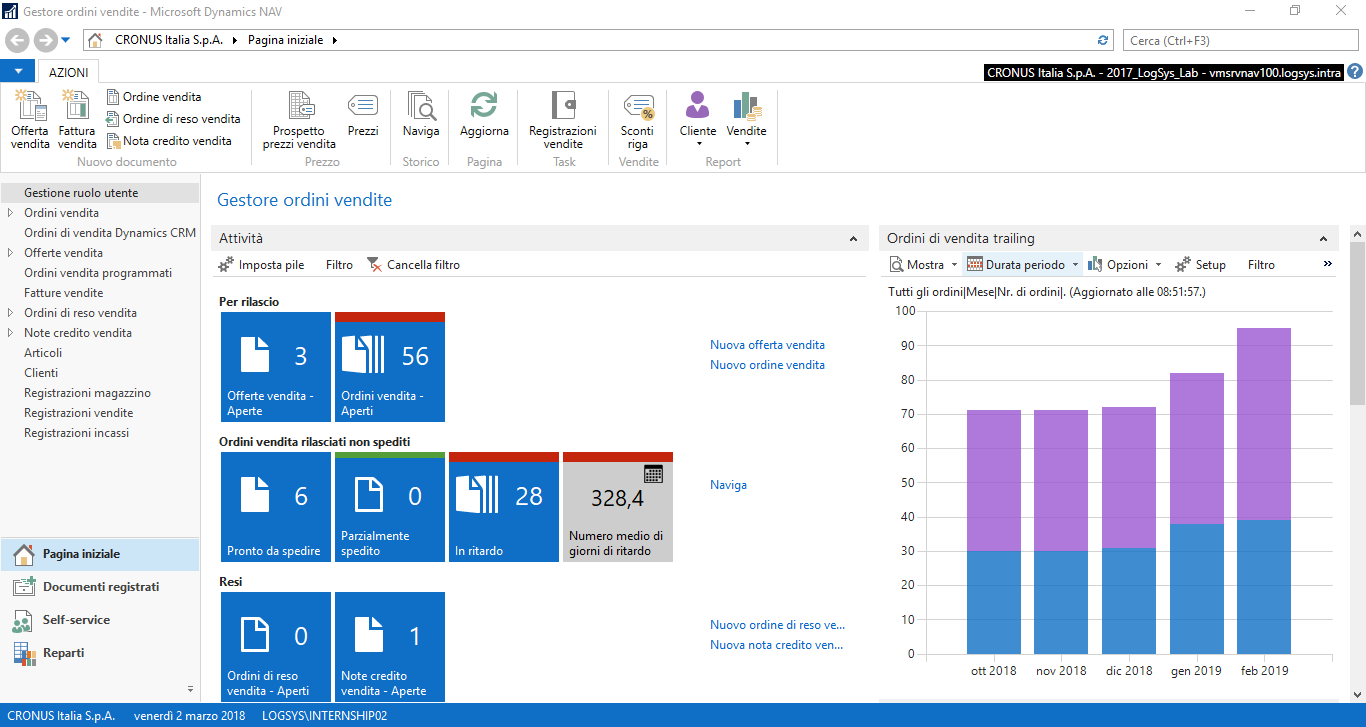
\includegraphics[width=1\textwidth]{images/NAVClient.png}
%\end{frame}

\begin{frame}
\frametitle{Class Diagram Client C\# 1}
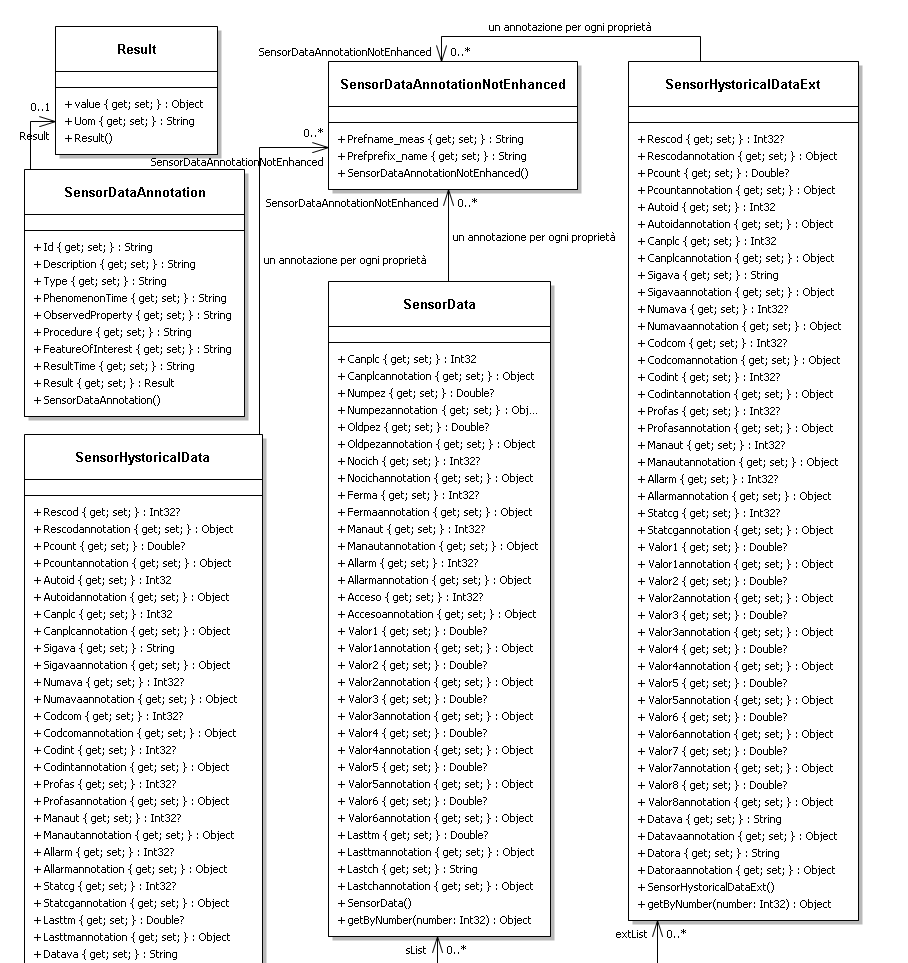
\includegraphics[width=0.65\textwidth]{images/ClassLibrary3v2part1.png}
\end{frame}

\begin{frame}
\frametitle{Class Diagram Client C\# 2}
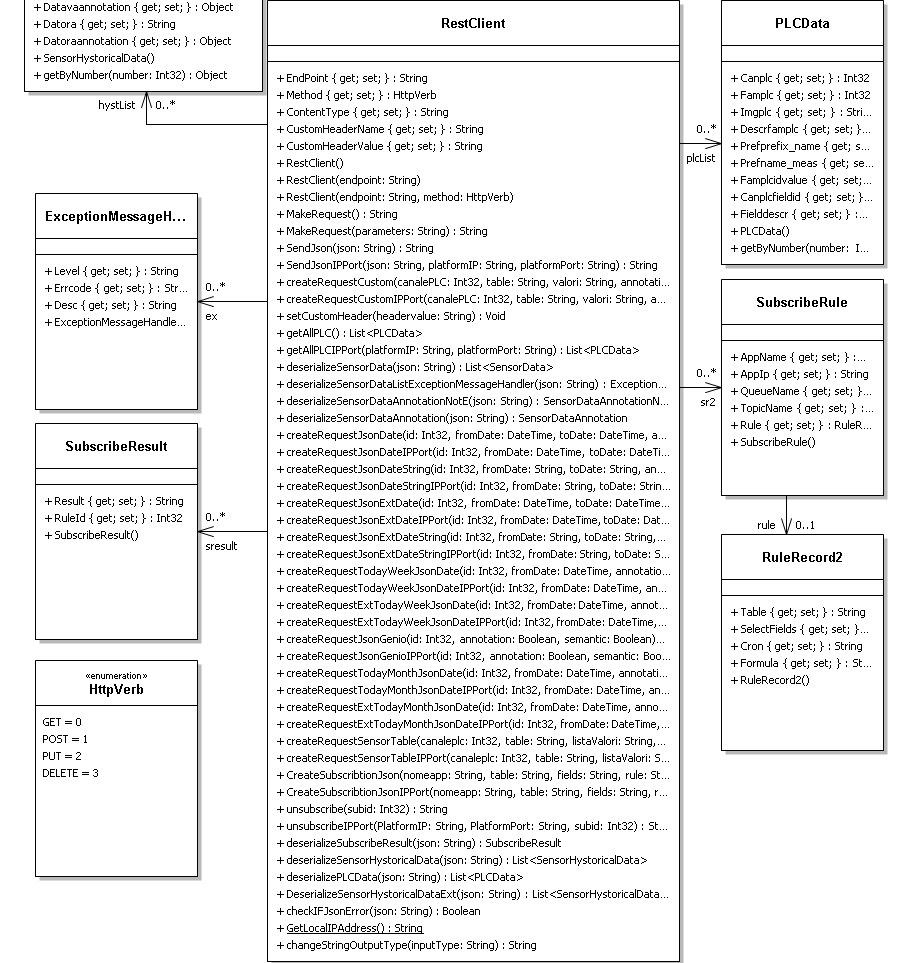
\includegraphics[width=0.65\textwidth]{images/ClassLibrary3v2part2.png}
\end{frame}

\begin{frame}
\frametitle{Ambiente di sviluppo (C/SIDE) NAV}
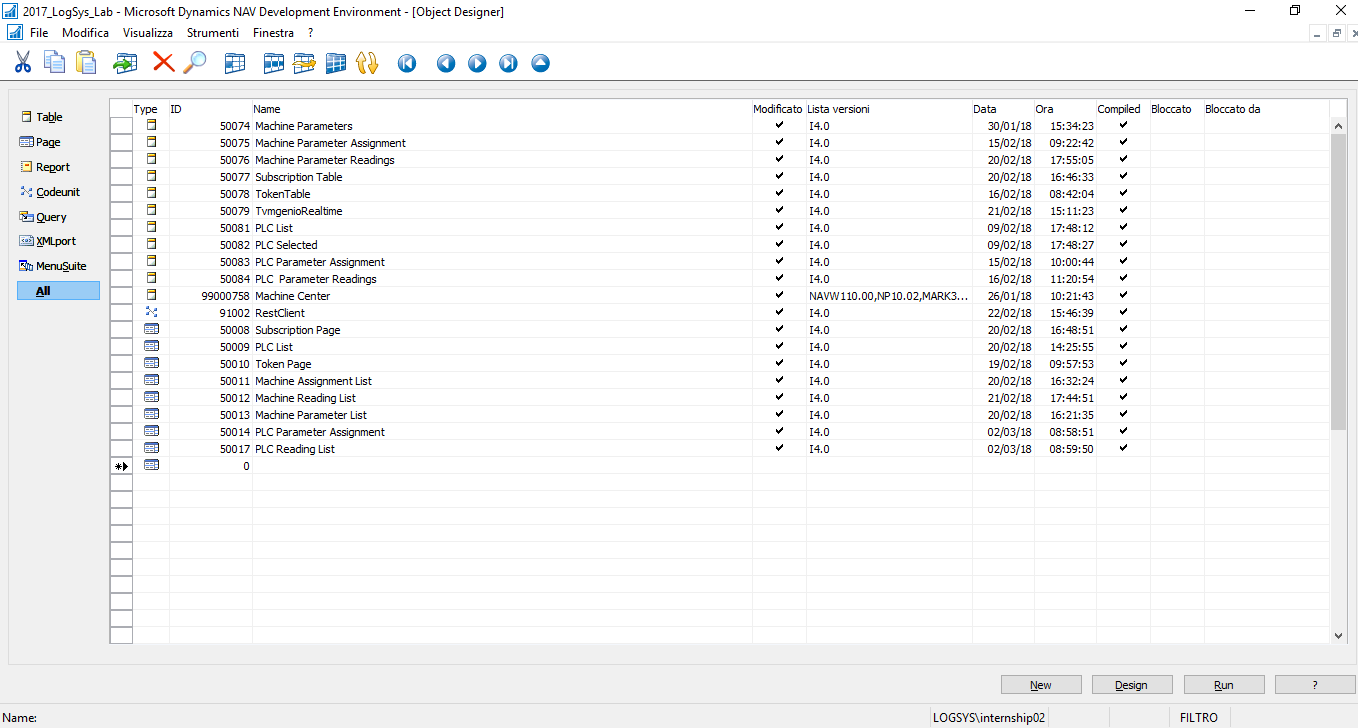
\includegraphics[width=1\textwidth]{images/NAVDevelopmentEnvironment.png}
\end{frame}


%\begin{frame}
%\frametitle{Lista delle funzioni della codeunit}
%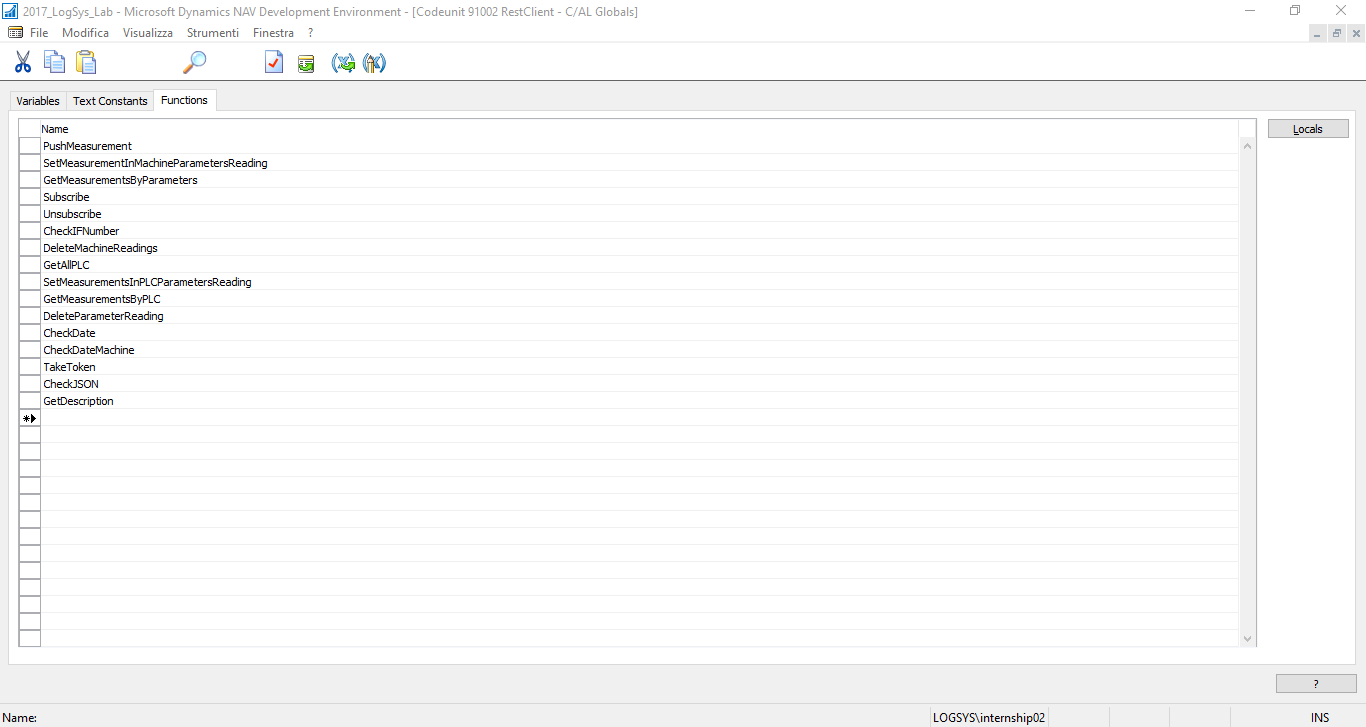
\includegraphics[width=1\textwidth]{images/NAVFunctionList.png}
%\end{frame}


%\begin{frame}
%\frametitle{La pagina Machine Center}
%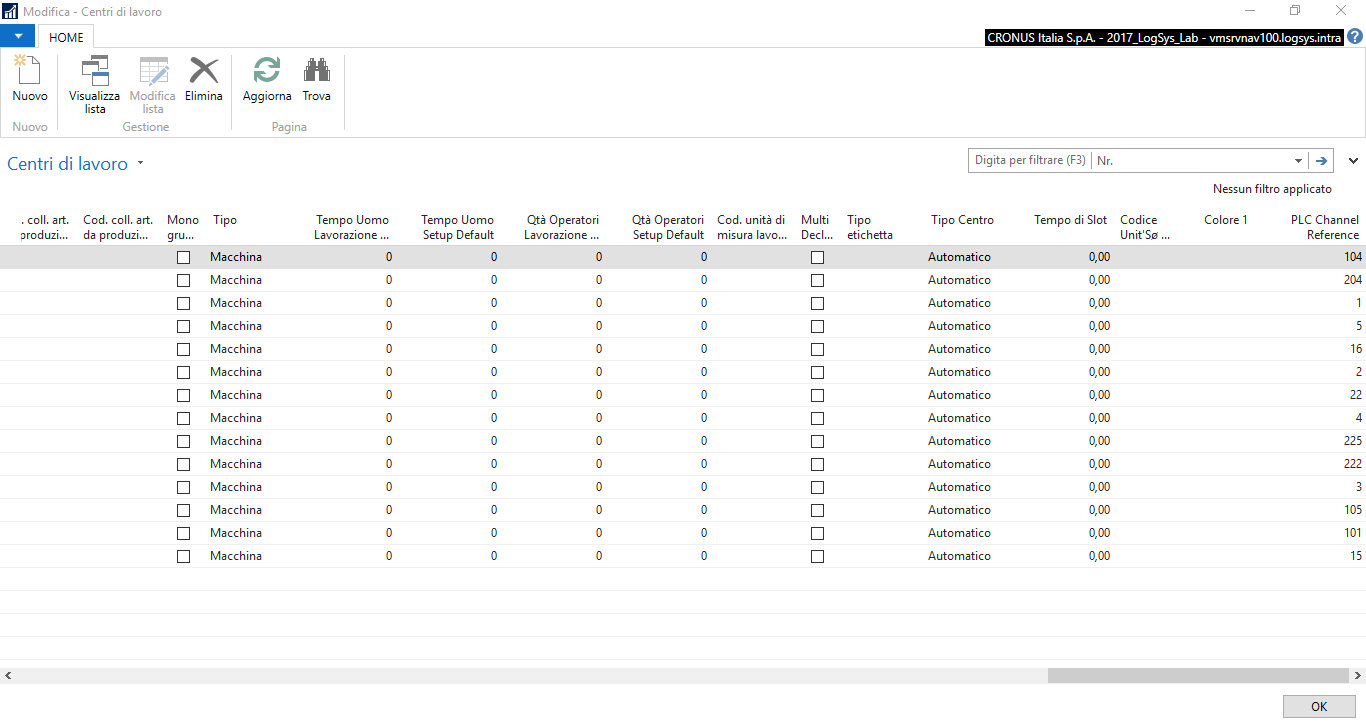
\includegraphics[width=1\textwidth]{images/MachineCenter.png}
%\end{frame}

\begin{frame}
\frametitle{La pagina Machine Assignment List}
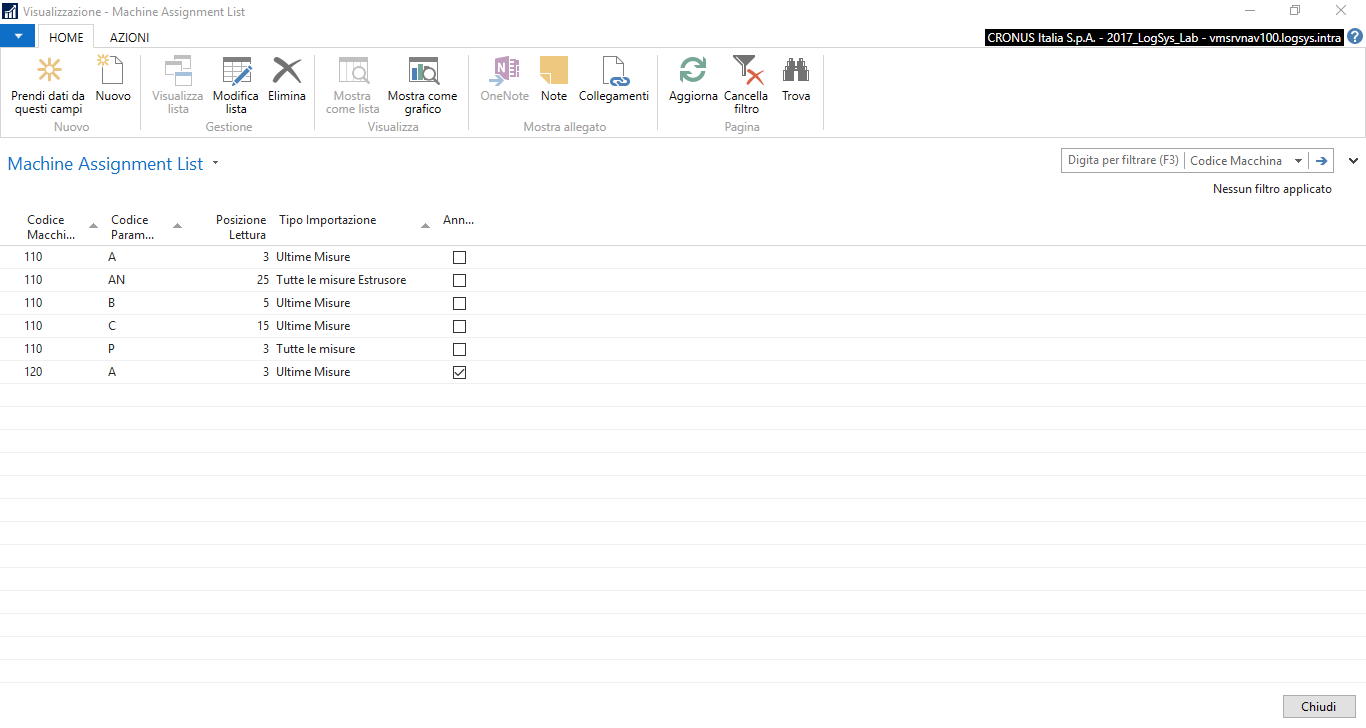
\includegraphics[width=1\textwidth]{images/MachineAssignmentList2.png}
\end{frame}


%\begin{frame}
%\frametitle{Lista con i parametri}
%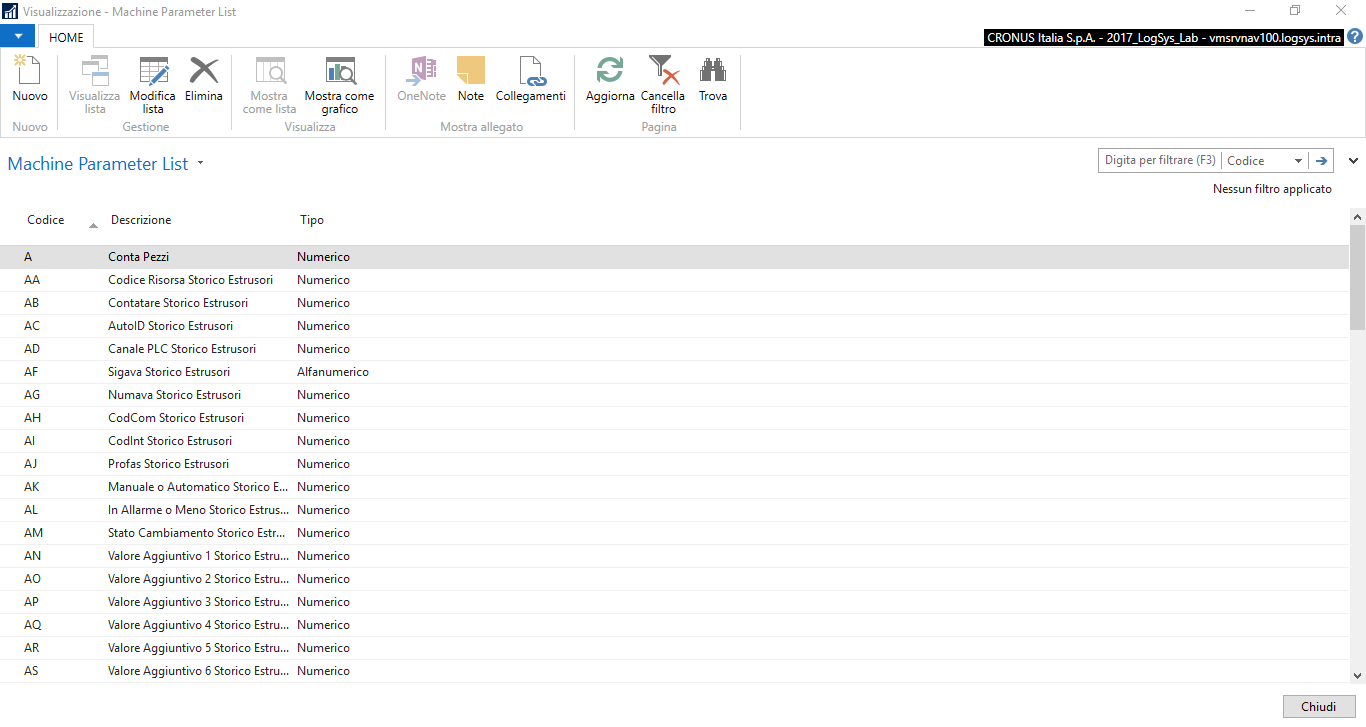
\includegraphics[width=1\textwidth]{images/MachineParameter.png}
%\end{frame}

%\begin{frame}
%\frametitle{Pagina del token}
%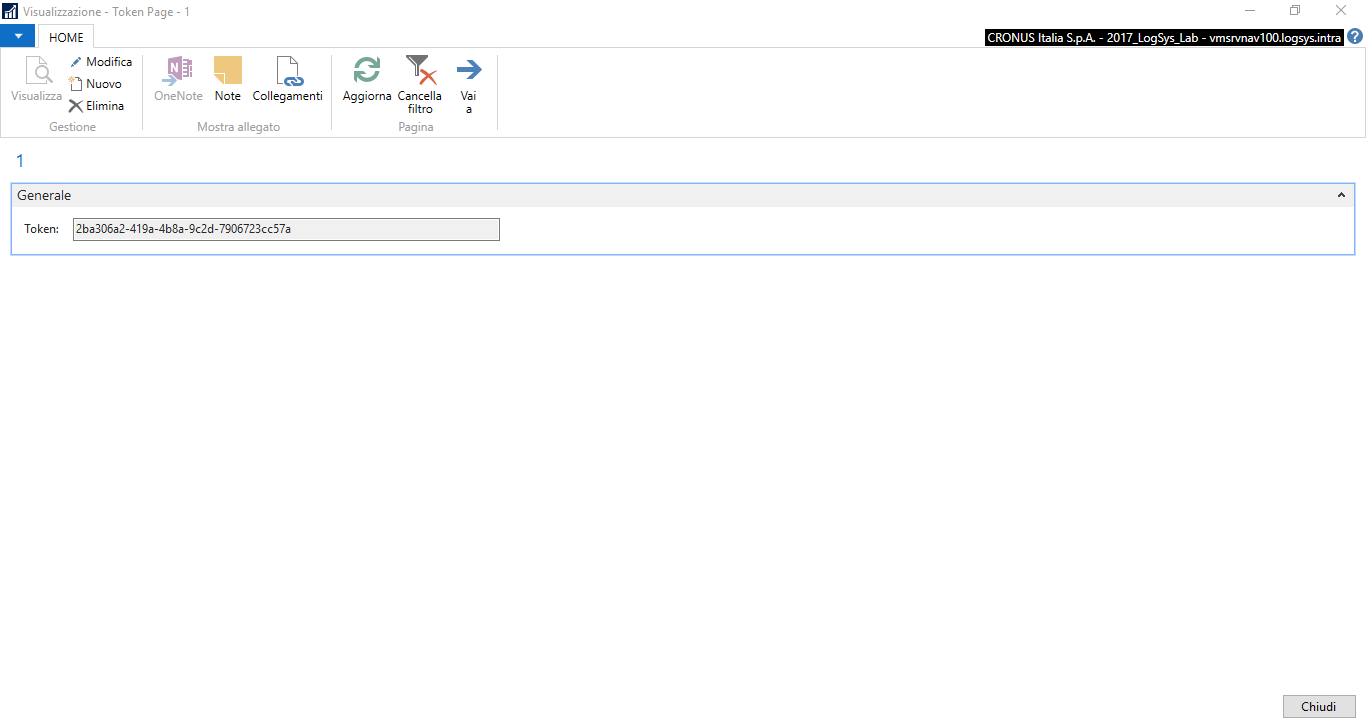
\includegraphics[width=1\textwidth]{images/tokenpage.png}
%\end{frame}



\begin{frame}
\frametitle{La pagina Machine Reading List}
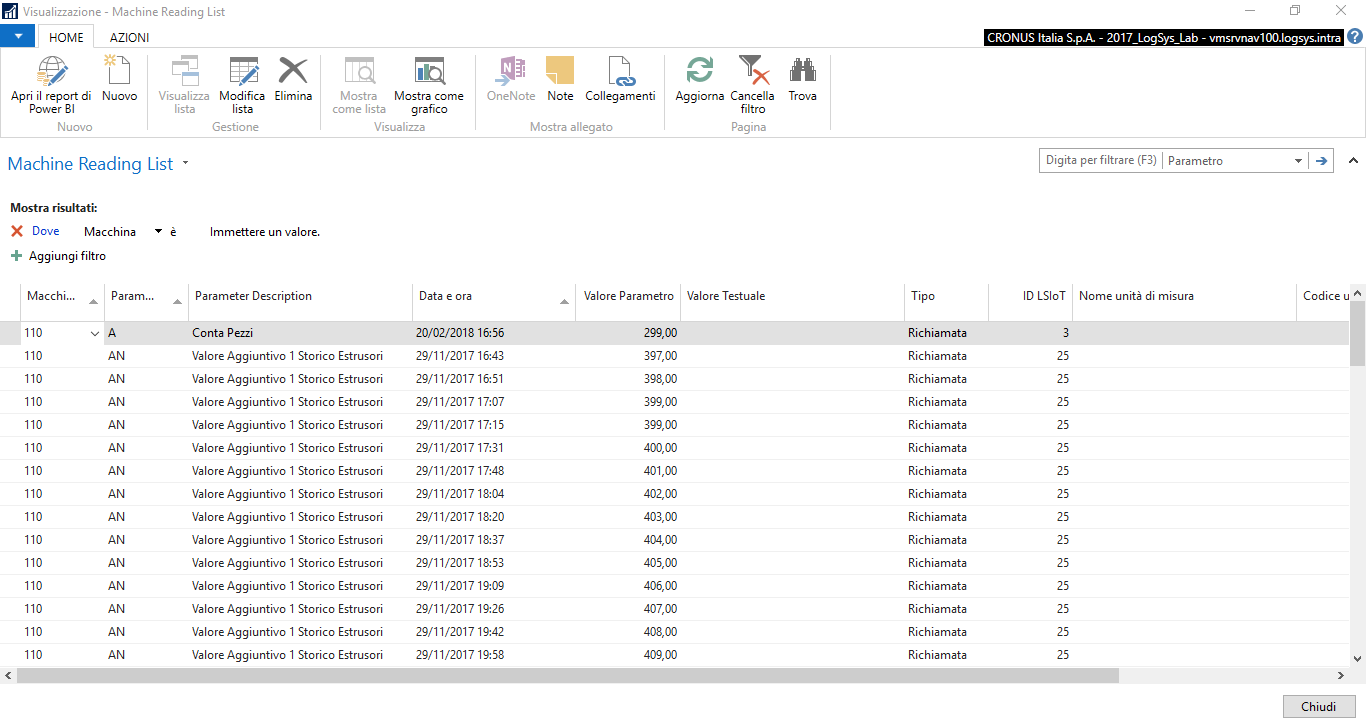
\includegraphics[width=1\textwidth]{images/MachineReadingList.png}
\end{frame}

\begin{frame}
\frametitle{Il report PowerBI nell'applicativo}
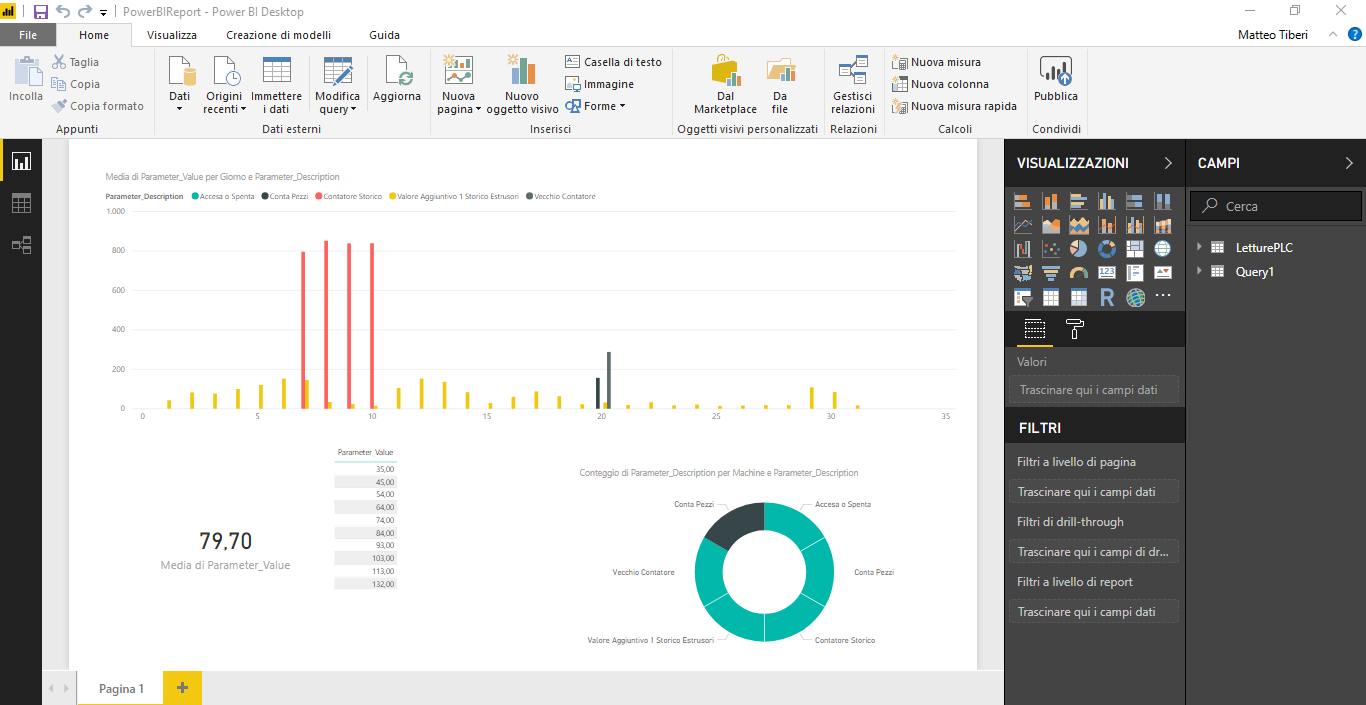
\includegraphics[width=1\textwidth]{images/PowerBI.png}
\end{frame}

\begin{frame}
\frametitle{Il report PowerBI esportato nel web}
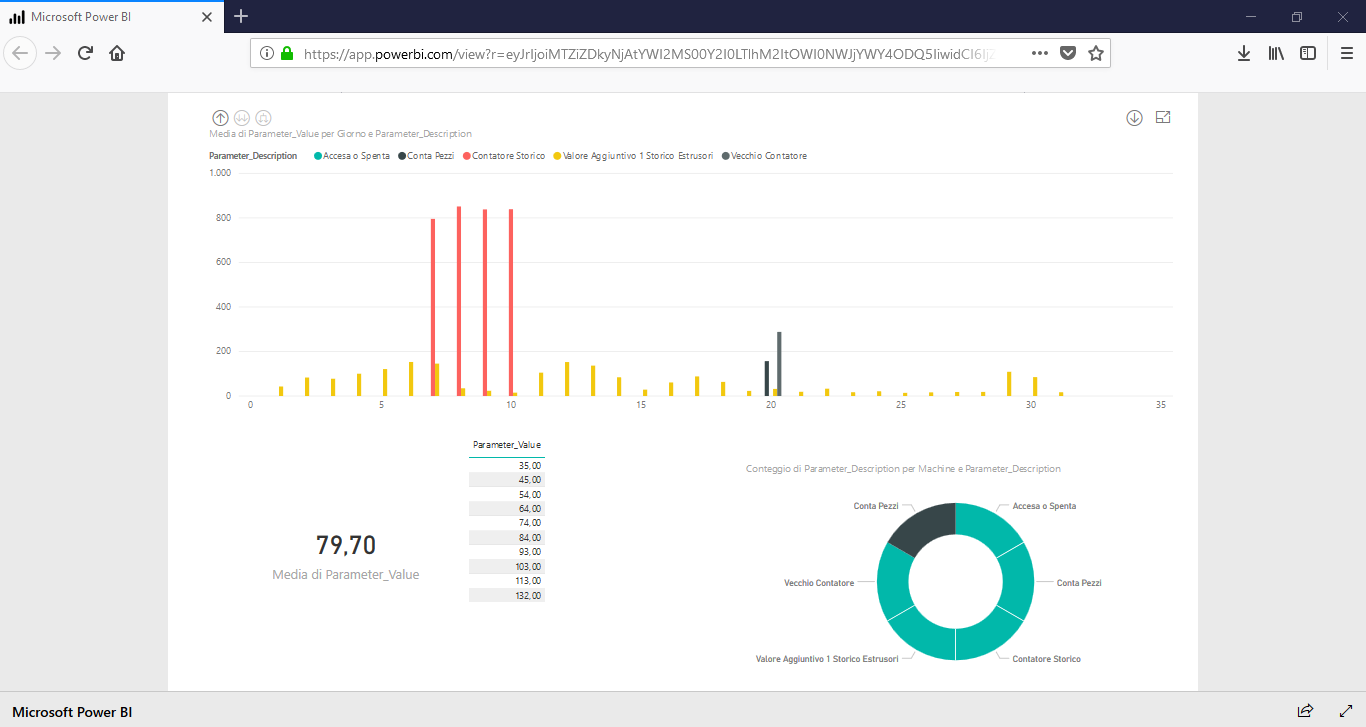
\includegraphics[width=1\textwidth]{images/ReportWEB.png}
\end{frame}

%\begin{frame}
%\frametitle{Metodo SetMeasurementPLC}
%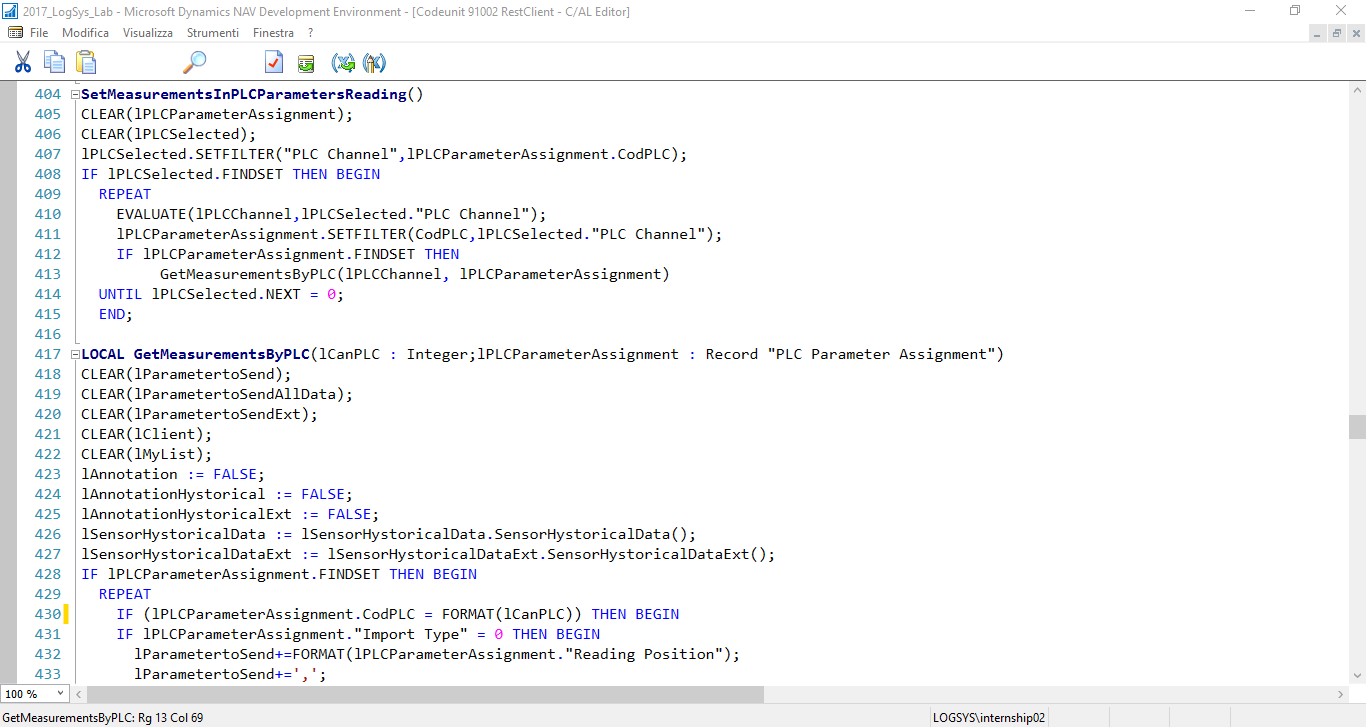
\includegraphics[width=1\textwidth]{images/NAVSetMesurament.png}
%\end{frame}

%\begin{frame}
%\frametitle{Metodo GetMeasurementPLC1}
%\includegraphics[width=1\textwidth]{images/NAVGetMesurament1.png}
%\end{frame}

%\begin{frame}
%\frametitle{Metodo GetMeasurementPLC2}
%\includegraphics[width=1\textwidth]{images/NAVGetMesurament2.png}
%\end{frame}

\begin{frame}
\frametitle{NAV servizi web}
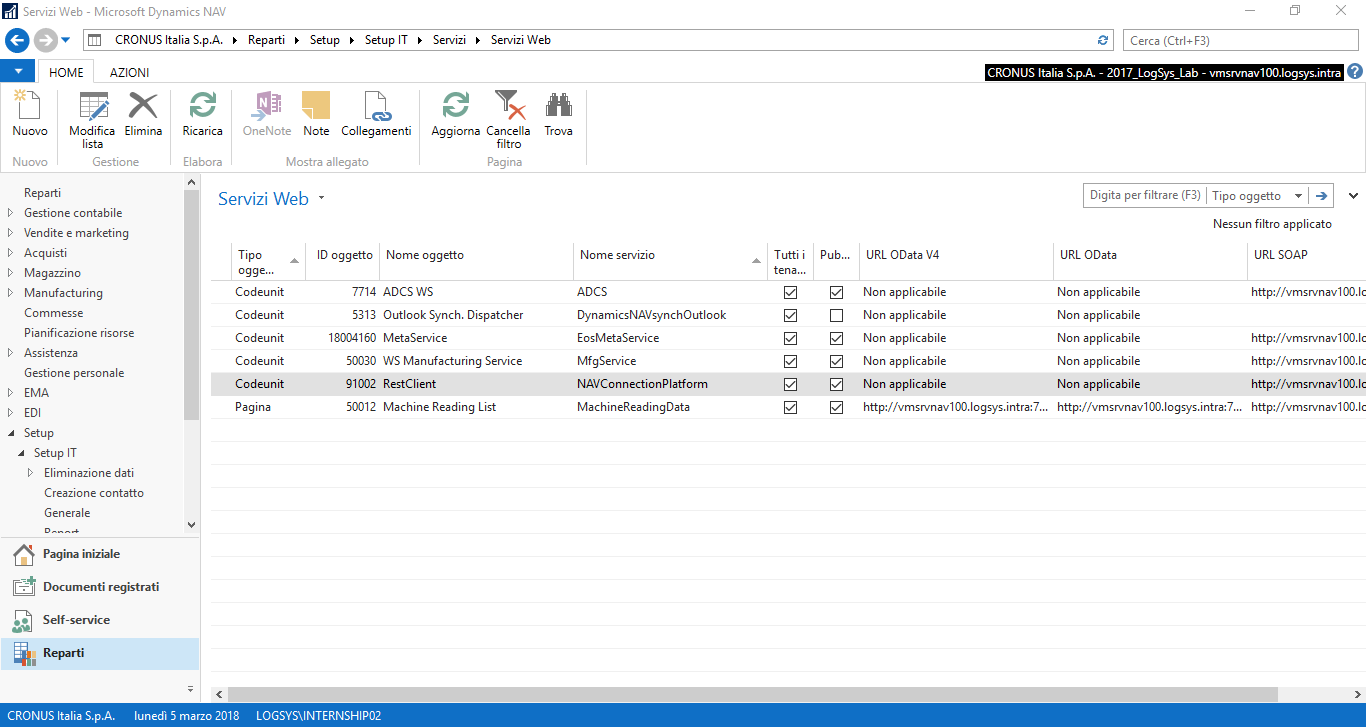
\includegraphics[width=1\textwidth]{images/NAVServiziWeb.png}
\end{frame}


\begin{frame}
\frametitle{NAV SubscriptionPage}
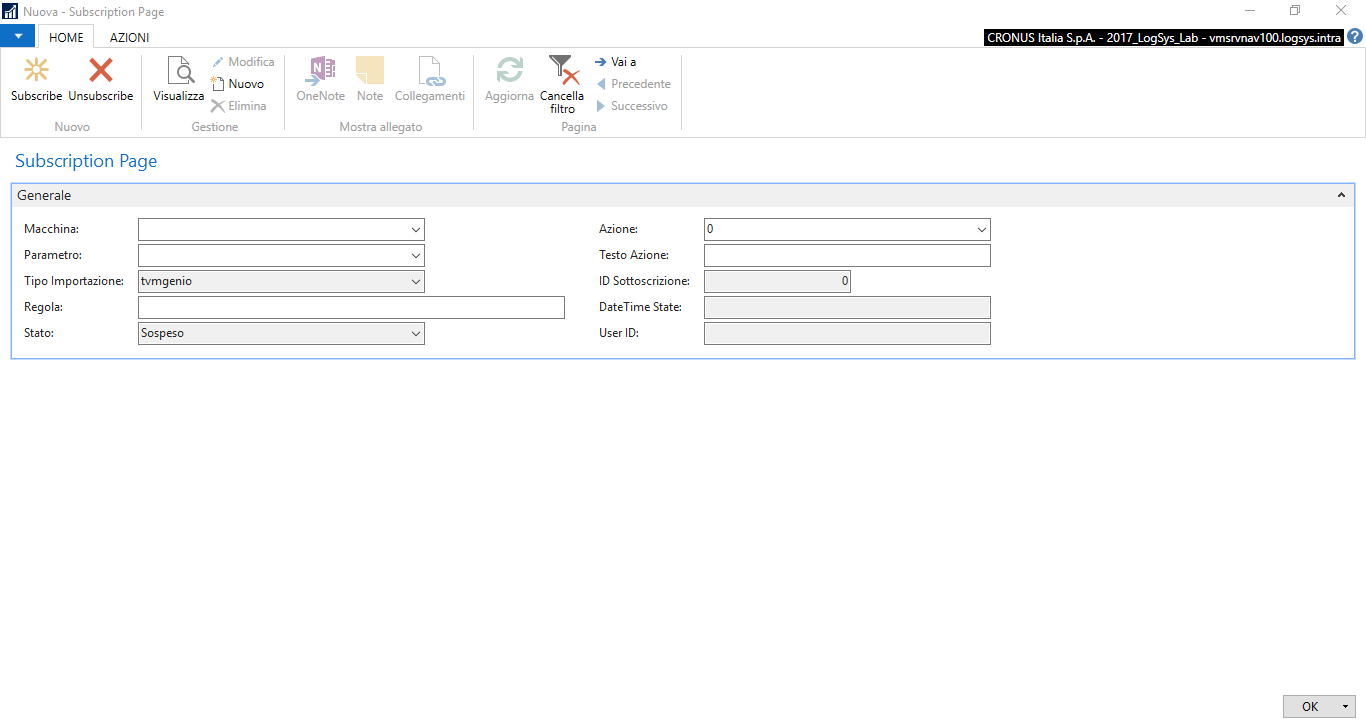
\includegraphics[width=1\textwidth]{images/NAVSubscriptionPage.png}
\end{frame}

\begin{frame}
\frametitle{Standard Observation and Measurement ISO 19156:2011}
\begin{itemize}
\item Standard basato sul concetto di osservazione, con implementazioni in formato XML e JSON
\begin{itemize}
\item Pensato per l'ambito geospaziale, il modello risulta astratto e applicabile nel case study
\end{itemize}
\item Concetto di osservazione generico specializzato in base al risultato (es. Measurement)
\begin{itemize}
%\item All'interno del case study non tutte le specializzazioni proposte vengono utilizzate
\item Solo alcune specializzazioni sono utilizzate nel case study
\end{itemize}
\item Al risultato di una osservazione specializzata viene poi associata un ontologia delle misure
\end{itemize}	
\end{frame}

\begin{frame}
\frametitle{Tabelle Annotazioni}
\includegraphics[width=1\textwidth]{images/AltreTabelleAnnotazioniMOD4.png}
\end{frame}

%\begin{frame}
%\frametitle{Metodo PushMeasurement 1}
%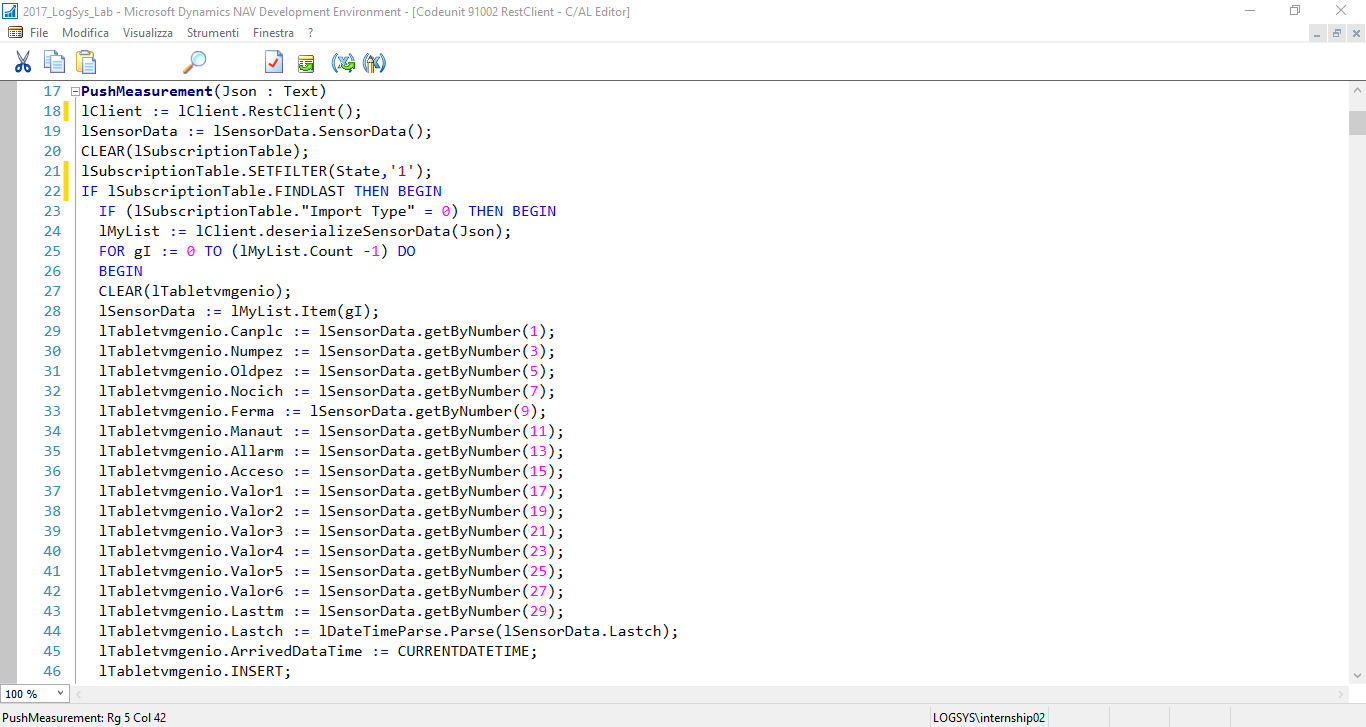
\includegraphics[width=1\textwidth]{images/NAVPushMeasuraments1.png}
%\end{frame}

%\begin{frame}
%\frametitle{Metodo PushMeasurement 2}
%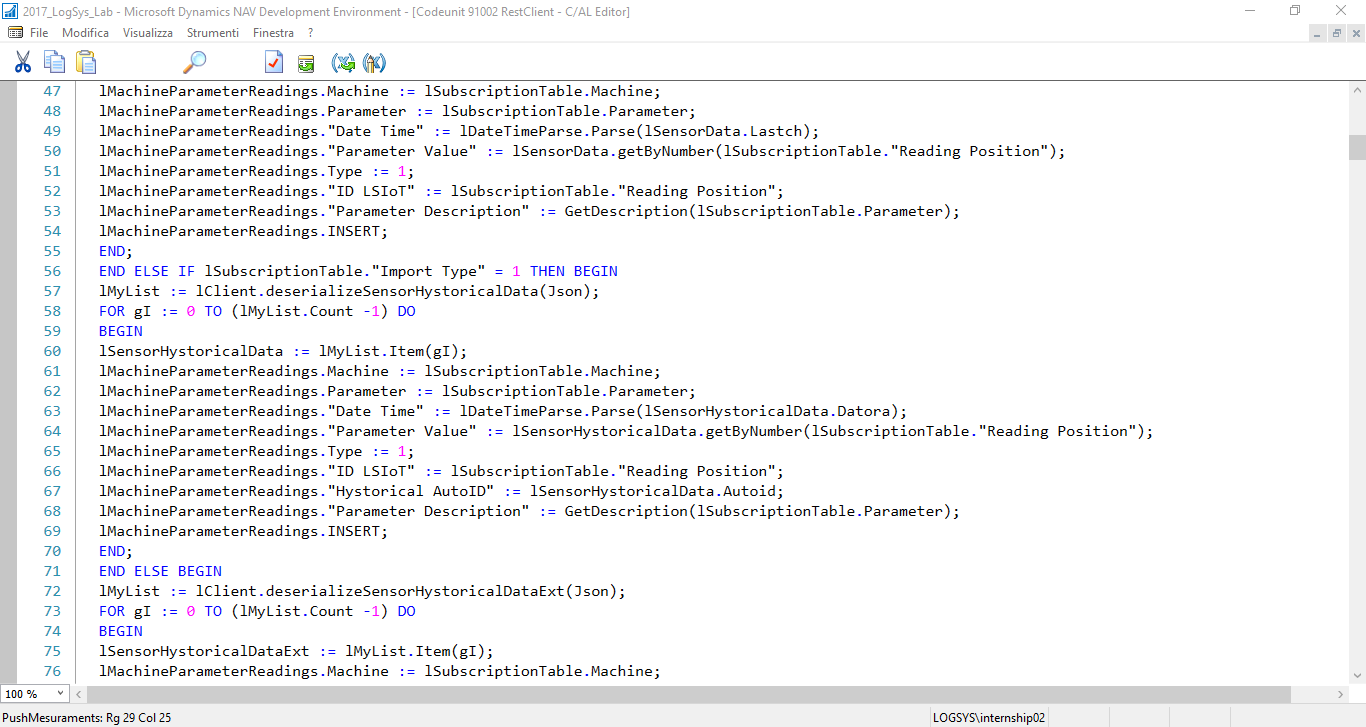
\includegraphics[width=1\textwidth]{images/NAVPushMeasuraments2.png}
%\end{frame}

%\begin{frame}
%\frametitle{Metodo PushMeasurement 3}
%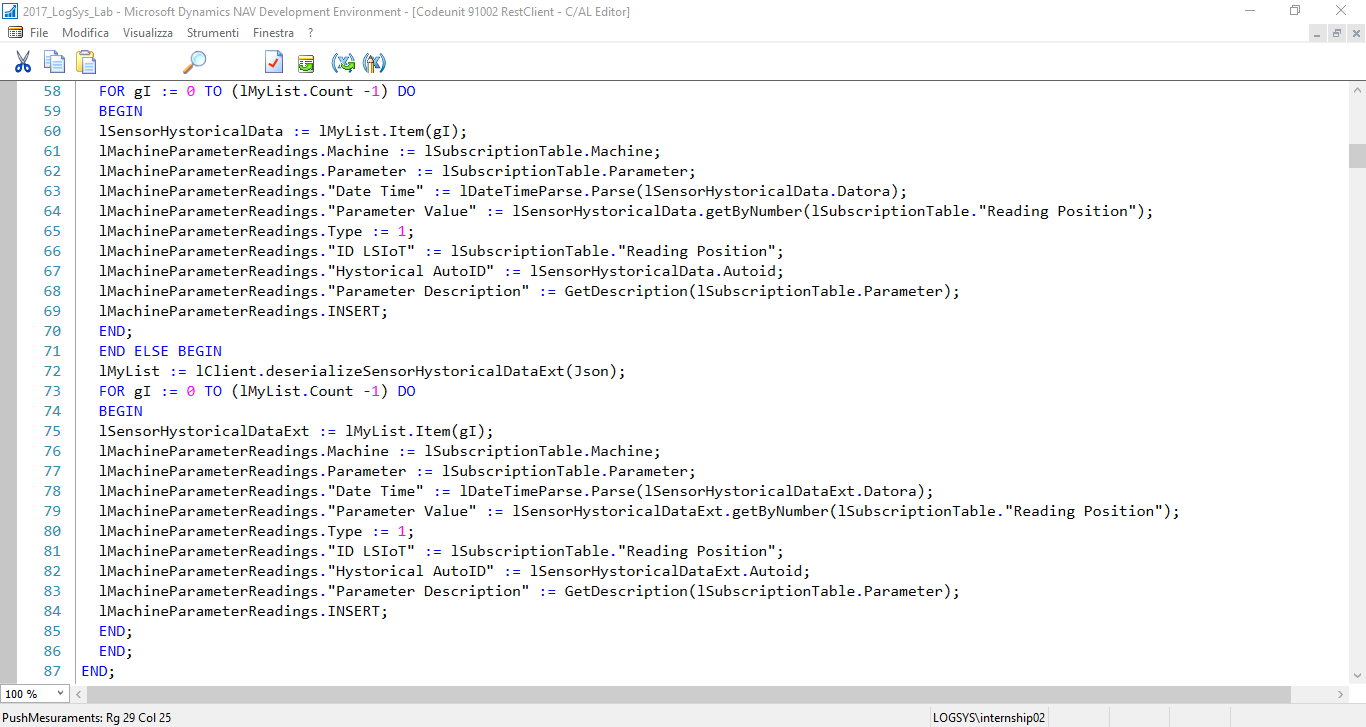
\includegraphics[width=1\textwidth]{images/NAVPushMeasuraments3.png}
%\end{frame}

\begin{frame}
\frametitle{Esempio XML}
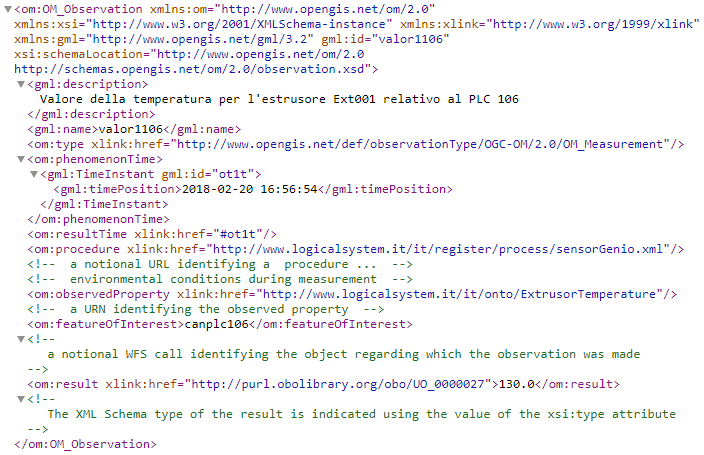
\includegraphics[width=1\textwidth]{images/TemperatureXML2.png}
\end{frame}

\begin{frame}
\frametitle{Esempio JSON}
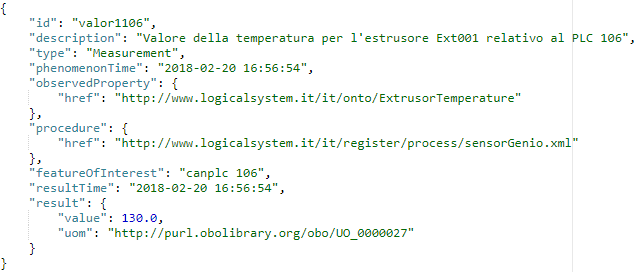
\includegraphics[width=1\textwidth]{images/TemperatureJSON.png}
\end{frame}

\begin{frame}
\frametitle{Grafico Misurazioni e misure}
\begin{figure}%
%\centering
\subfloat{{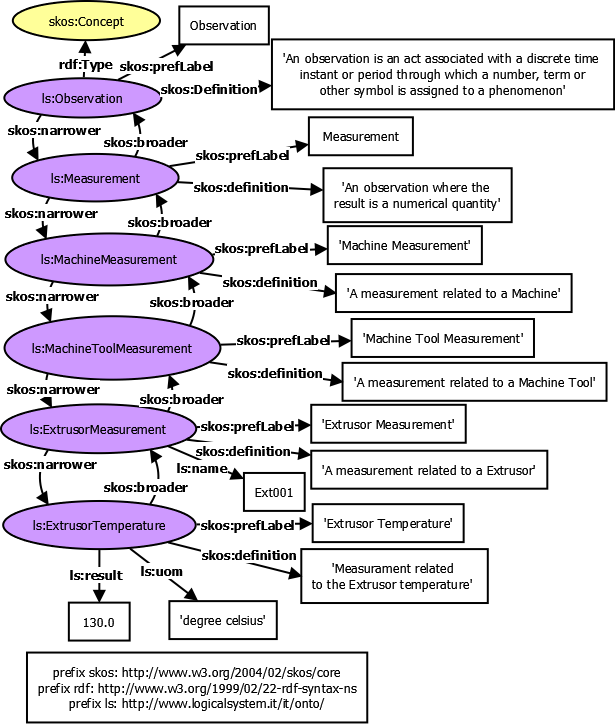
\includegraphics[width=0.565\columnwidth]{images/TempExample2.png} }}%
%\qquad
\hfill
\subfloat{{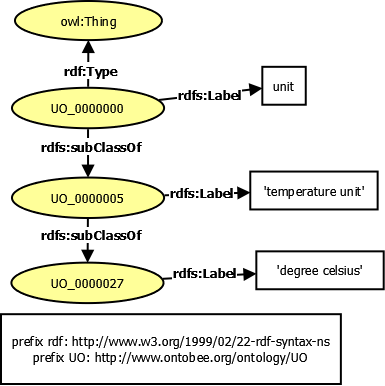
\includegraphics[width=5cm]{images/celsius.png} }}%
%
%
\end{figure}
\end{frame}

%\begin{frame}
%\frametitle{Grafico Misurazioni}
%\begin{center}
%	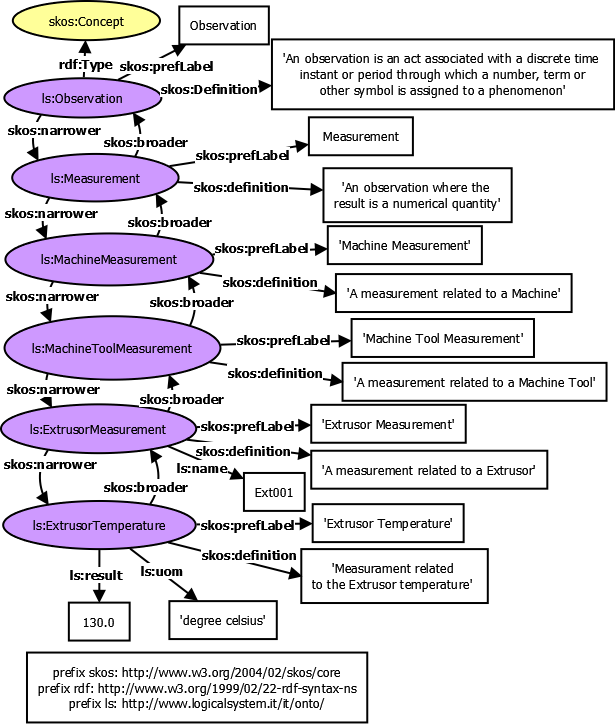
\includegraphics[width=0.6\textwidth]{images/TempExample2.png}
%\end{center}
%\end{frame}

%\begin{frame}
%\frametitle{Grafico Misure}
%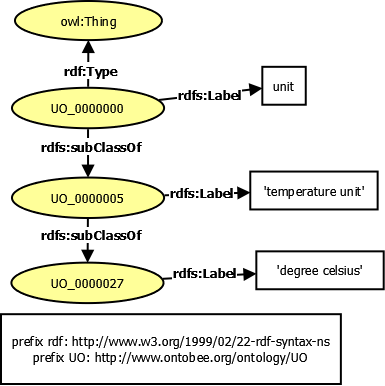
\includegraphics[width=0.6\textwidth]{images/celsius.png}
%\end{frame}

\begin{frame}
\frametitle{Pagina web ontologia}
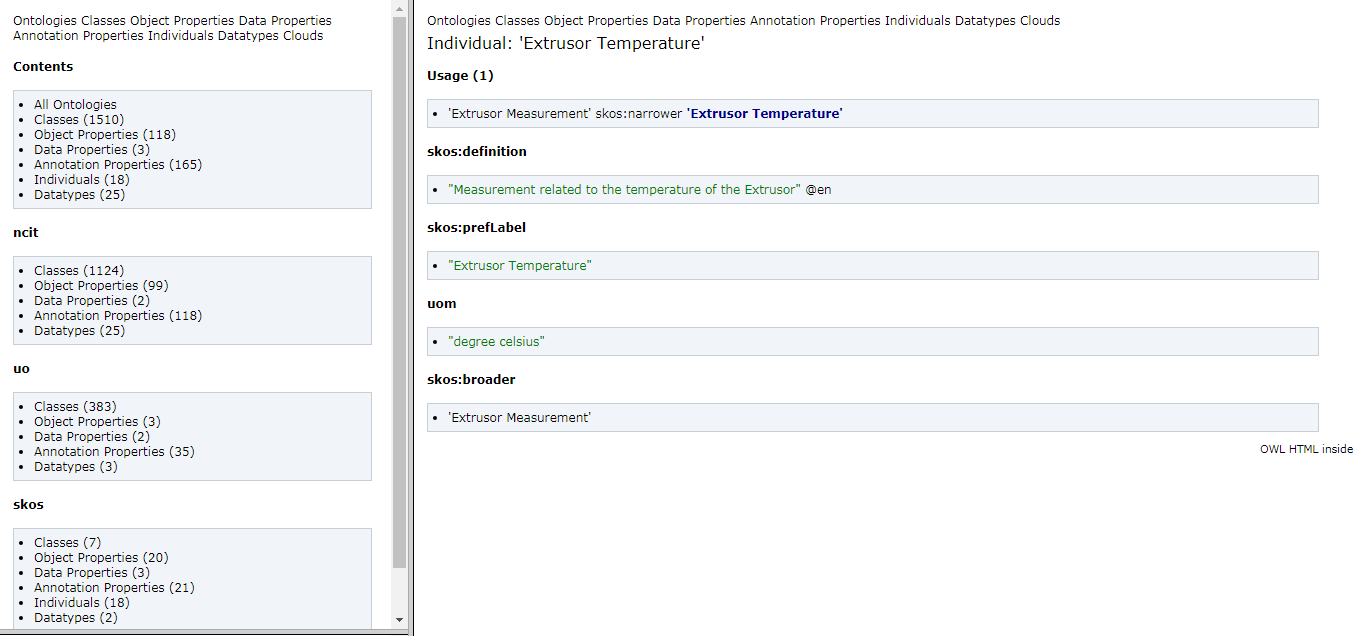
\includegraphics[width=1\textwidth]{images/ExtrusorTemperature2.png}
\end{frame}

\begin{frame}
\frametitle{JSON con annotazione semantica}
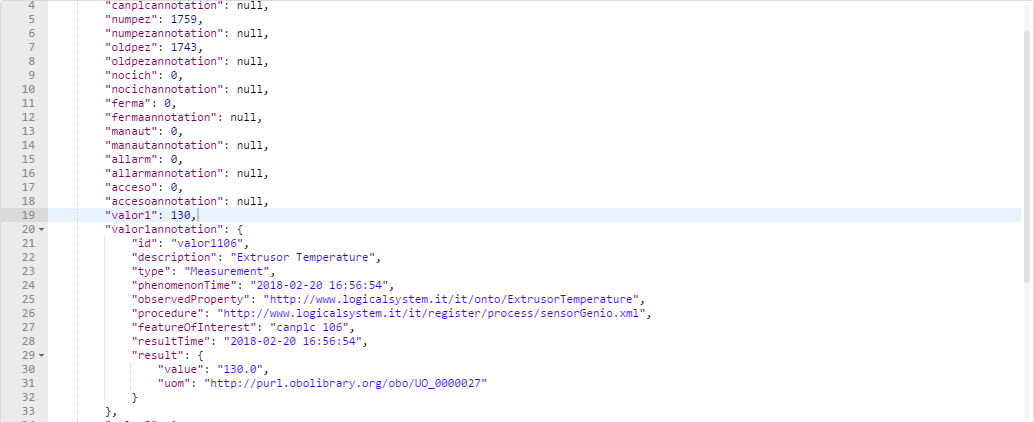
\includegraphics[width=1\textwidth]{images/JSONRestituito.png}
\end{frame}


\begin{frame}
\frametitle{Conclusioni}
\begin{itemize}
\item L'integrazione tra NAV e la piattaforma ha avuto esito positivo tramite uso del client C\# 
\begin{itemize}
\item Permettendo agli utenti un semplice utilizzo dei servizi
\end{itemize}
%\item Il report PowerBI è disponibile tramite NAV
%\begin{itemize}
%	\item Permettendo agli utenti una visualizzazione grafica dinamica dei dati ricevuti
%\end{itemize}
\item L'ontologia delle misurazioni e delle misure è stata implementata
\begin{itemize}
\item In modo da avere una descrizione dei dati ottenuti dai servizi
\end{itemize}

\end{itemize}	
\end{frame}


\end{document}